\documentclass[Ex4_Zusammenfassung.tex]{subfiles}


\lehead{\pagemark}
\rehead{\headmark}
\lohead{\pagemark}
\rohead{\headmark}
\pagestyle{scrheadings}

\begin{document}
\chapter{Wechselwirkung von Teilchen und Strahlung mit Materie}
\textbf{von \anton, \soeren \& \chris}\\

Bei der Wechselwirkung von Teilchen mit Atomen oder Molekülen können folgende elementare Prozesse ablaufen:
\begin{itemize}
	\item Rayleigh--Streuung, Thomson--Streuung
	\item Anregung oder Ionisation von Hüllenelektronen
	\item Ablenkung geladener Teilchen im Coulomb--Feld des Kerns, die zur Emission von Bremsstrahlung führt
	\item Compton--Streuung
	\item Emission von Cerenkov--Strahlung, wenn geladene Teilchen ein Medium mit Brechungsindex n schneller als die Lichtgeschwindigkeit $\frac{c}{n}$ durchlaufen
\end{itemize}
All diese Effekte können einzeln oder in Kombination zum Nachweise der Teilchen ausgenutzt werden, wobei der vorletzte Prozess einen wesentlich kleineren Wirkungsquerschnitt hat und erst bei großen Energien eine merkliche Rolle spielt.
Ein Teilchen mit einer kinetischen Energie im $\si{keV}-\si{MeV}$--Bereich verliert bei der Ionisation eines Atoms oder Moleküls nur einen Bruchteil seiner Energie. Es kann daher bei seinem Weg durch den Detektor viele Atome anregen. Der spezifische Energieverlust pro Längeneinheit $\derive{E}{x}$ hängt außer von der Art und Dichte der Detektormaterie stark von der Art des ionisierenden Teilchens und von seiner Energie ab.

\begin{figure}[H]
	\centering
	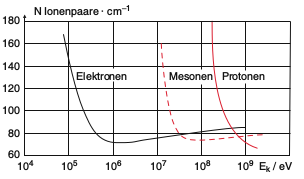
\includegraphics[width=8cm]{Ionisationsplot2.png}
	\caption{Spezifische Ionisierung (Zahl der pro cm Weg gebildeten Ionenpaare) für Elektronen, Protonen und $\pi$--Mesonen in Luft als Funktion der kinetischen Energie.}
\end{figure}
\section{Energieverlust von geladenen schweren Teilchen}
Wir betrachten ein Teilchen der Ladung $Z_1 \cdot e $, das durch die Elektronenhülle eines Atoms fliegt. Ist die Energie des Teilchens groß gegen die Bindungsenergie der Elektronen in der Atomhülle, so ist der beim Stoß des schweren Teilchens auf \textbf{ein} Elektron  übertragene relative Impuls $\frac{\Delta p}{p}$ klein. Die Teilchenbahn kann durch eine Gerade angenähert werden, und die Elektronen können als frei angesehen werden.
Dieses Modell wird mathematisch durch die Bethe--Formel beschrieben:
\begin{equation}\label{bethe-formel}
	\derive{E}{x} = - \frac{4 \pi Z_1^2 e^2 e^2 n_e}{v^2 m_e} \cdot \left( \ln \frac{2 m_e v^2}{I} - \ln \lp 1-\beta^2\rp - \beta^2 \right)
\end{equation}
wobei $I \approx Z_1\cdot 10\si{eV}$ das mittlere Anregungspotential ist.

Man sieht hieraus, dass der spezifische Energieverlust $\derive{E}{x}$ proportional zur Elektronendichte $n_e$ im Detektor ist und mit dem Quadrat der Teilchenladung $Z_1 \cdot e$ ansteigt, aber umgekehrt proportional zum Quadrat der Ionengeschwindigkeit $v$ abnimmt. Der spezifische Energieverlust geladener schwerer Teilchen $\derive{E}{x} $ hängt von ihrer Energie E ab wie $ \frac{1}{E} \cdot \ln \lp \frac{E}{I} \rp $. Er sinkt also schwach mit steigender Energie.

\section{Energieverlust von Elektronen}
\subsection{Anregung und Ionisation}
Für leichte Teilchen (Elektronen, Positronen) mit $v \ll c$ kann man die Richtungsablenkung bei Stößen mit der Elektronenhülle nicht mehr vernachlässigen. Ein parallel einfallender Strahl wird daher wesentlich stärker durch Streuung diffus. In diesem Fall wurde der spezifische Energieverlust durch Ionisation von Bethe berechnet zu: 
\begin{equation}
	\derive{E}{x} \approx \frac{4\pi Z_1 e^4 n_e }{m_e v^2} \cdot  \ln \frac{m_e v^2}{2 I }
\end{equation}
Der Vergleich mit (\ref{bethe-formel}) zeigt, dass bei gleicher Geschwindigkeit $v$ der spezifische Energieverlust pro Weglänge für schwere Teilchen (Masse $m_S$) und Elektronen (Masse $m_e$) gleich ist, bei gleicher Energie jedoch für Elektronen um den Faktor $\frac{m_e}{m_S} $ kleiner ist. Die Reichweite von Elektronen ist deshalb trotz der größeren Streuung wesentlich größer als die von schweren Teilchen der gleichen Energie. Für Teilchen mit relativistischen Energien sind dagegen die Unterschiede für $\derive{E}{x}$ zwischen Elektronen und schweren Teilchen nur noch klein. 

\begin{figure}[H]
	\centering
	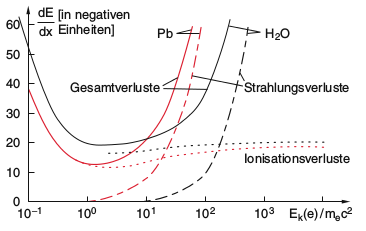
\includegraphics[width=9cm]{Strahlungsverluste2.png}
	\caption{Ionisationsverluste,Strahlungsverluste und Gesamtverluste $ \derive{E}{x} $ (in relativen Einheiten) von Elektronen in Blei (rote Kurven) und Wasser (schwarze Kurven) als Funktion der Elektronenenergie}
\end{figure} 

\subsection{Bremsstrahlung}
Durch die Ablenkung im Coulomb-Feld der Atomkerne erfahren die Elektronen eine negative Beschleunigung und strahlen deshalb elektromagnetische Wellen ab, deren Leistung proportional zum Quadrat der Beschleunigung ist. Die Rechnung ergibt für den Strahlungsenergieverlust pro Weglänge eines Elektrons mit der kinetischen Energie $E_e$ in einem Medium mit der Atomdichte $n_a$ und der Kernladung $Ze$
\begin{equation}
	\left( \derive{E}{x} \right)_{Str} = \frac{4 n_a Z^2 \alpha^3 (\hslash c)^2 E_e}{m_e^2 c^4} \cdot \ln \frac{a(E)}{Z^{\nicefrac{1}{3}}} 
\end{equation}
wobei $\alpha = \frac{e^2}{\hslash c} $ die Feinstrukturkonstante ist und $a(E)$ ein numerischer Faktor, der angibt, bei welchem Stoßparameter das Elektron noch nahe genug am Kern vorbei läuft, um genügend abgelenkt zu werden. Die Strahlungsverluste pro Weglänge nehmen also etwas stärker als linear mt der Energie der Elektronen zu und überwiegen bei großen Energien die Ionisationsverluste.

Die Länge nach der die Energie des Elektrons durch Strahlungsverluste auf $\frac{1}{e} $ abgeklungen ist heißt die Strahlungslänge 
\begin{equation}
	X_0 = \left( \derive{E}{x} \cdot \frac{1}{E_e} \right)^{-1}
\end{equation}

\begin{figure}[H]
	\centering
		\begin{tikzpicture}
		\draw [->, >=latex] (-1,-2) -- (4, -2) node [midway, below] {$t$};
			\begin{feynman}
				\vertex (e1) {$e^-$};
				\vertex [right = of e1] (a);
				\vertex [below left = of a] (core) {$\bigotimes$};
				\vertex [above right = of a] (e2) {$e^-$};
				\vertex [below right = of a] (gammatmp);
				\vertex [right=1cm of gammatmp] (gamma) {$\gamma$};
				\vertex [right=0.4cm of a] (atemp);
				\vertex [above=0.4cm of atemp] (a2);
			
				\diagram* {
					(e1) -- [fermion] (a) -- [fermion] (e2),
					(gamma) -- [photon] (a2) ,
					(a) -- [photon, edge label=$\gamma$] (core),
						};
			\end{feynman}
		\end{tikzpicture}
		\caption{Feynman--Diagramm für Bremsstrahlung von Elektronen. Es wird ein Atomkern $\bigotimes$ für die gleichzeitige Impuls-- und Energieerhaltung benötigt.}
\end{figure}

\section{Wechselwirkung von radioaktiver Strahlung mit Materie}
\subsection{$\alpha$-Strahlung}
$\alpha$-Strahlung besteht aus schweren Heliumkernen und verhält sich somit wie schwere Teilchen mit Materie. Wir betrachten hier die Zunahme des Energieverlusts bei kleineren Energien.

\begin{figure}[H]
	\centering
	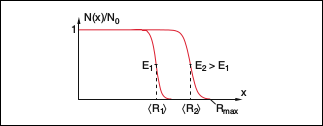
\includegraphics{alpha-Strahlung_Reichweite.png}
	\caption{Reichweite von $\alpha$-Teilchen in Luft, dargestellt als relative Abnahme der Anzahl}
\end{figure}
Die Weglänge von $\alpha$-Teilchen ist scharf begrenzt.

\subsection{$\beta$-Strahlung}
$\beta^-$-Strahlung besteht aus Elektronen, für die wir das Wechselwirkungsverhalten schon kennen. 

$\beta^+$-Strahlung besteht aus Positronen, die beim Durchdringen von Materie sehr bald auf ihr Antiteilchen, das Elektron, treffen und durch Annihilation meist 2 Photonen entstehen und es zu $\gamma$-Strahlung kommt.

\subsection{$\gamma$--Strahlung}
Für den Nachweis von $\gamma$-Strahlung sind die folgenden Wechselwirkungsprozesse von besonderer Bedeutung:
\begin{itemize}
	\item elastische Streuung (Rayleigh-- und Thomson-Streuung)
	\item Inelastische Streuung (Compton--Effekt)
	\item Absorbtion in der Elektronenhülle (Photoeffekt)
	\item Absorbtion durch Atomkerne (Kern--Photoeffekt)
	\item Erzeugung von Teilchen durch $\gamma$--Quanten (Paarbildung)
\end{itemize}
Die Dominanz dieser einzelnen Effekte hängt von der Energie des Photons ab.

\subsubsection{Rayleigh--Streuung \& Thomson--Streuung}
Relevant bei \textbf{kleinen Energien} ($h \nu < I $). 

Es wird ein Photon elastisch an einem geladenen freien oder schwach gebundenem Teilchen gestreut. Das geladene Teilchen wird durch das Feld einer elektromagnetischen Welle zu harmonischen Schwingungen angeregt indem durch das elektrische Feld ein Dipolmoment induziert wird. Da diese Oszillation eine beschleunigte Bewegung ist, strahlen die Teilchen gleichzeitig Energie in Form einer elektromagnetischen Welle gleicher Frequenz ab (Dipolstrahlung). Man sagt die Welle wird gestreut. \\ 

\textbf{Rayleigh--Streuung} \\ 

 Die Energie des Photons ist zu klein, um das Atom anzuregen. Die Streuung findet also nur an gebundenen Elektronen statt. Für den Wirkungsquerschnitt gilt bei diesem Prozess
\begin{equation}
\sigma \propto \nu^4
\end{equation}

\textbf{Thomson--Streuung} \\

Thomson--Streuung tritt auf, solange die Energie des einfallenden Photons klein genug ist (Wellenlänge des Photons ist viel größer als Atomradius). Bei kürzeren Wellenlängen, also höheren Energien, muss der Rückstoß des Elektrons berücksichtigt werden (Compton--Streuung). Die Thomson--Streuung ist also der Grenzfall der Compton--Streuung für kleine Photonenenergien.  Die Größenordnung des Wirkungsquerschnitts dieser Wechselwirkung lässt sich durch den Thomson--Querschnitt beschreiben:
\begin{equation}
\sigma_{T} = 6.65 \cdot 10^{-29}  m 
\end{equation}

\subsubsection{Gemeinsamkeiten}
\begin{itemize}
\item Beide Arten der Streuung beruhen auf einem elastischen Stoß.
\item Beide Streuprozesse werden als kohärent bezeichnet, da sie die Kohärenz der elektromagnetischen Strahlung erhalten. 

(Kohärenz: Auslenkung zweier Wellen ändert sich zeitlich auf dieselbe Weise bis auf eine Phasenverschiebung)
\end{itemize}

\subsubsection{Unterschied} 
Rayleigh-Streuung geschieht an einem gebundenen Elektron, Thomson-Streuung an einem freien bzw. sehr schwach gebundenen Elektron.

\subsubsection{Compton--Effekt}
Bei \textbf{höheren} Photoenergien ($ h \nu \gg I$) wird der Compton--Effekt wichtig. Ein Photon streut an einem Teilchen und gibt einen Teil seiner Energie an das Teilchen ab. Durch diesen Energieverlust wird die Wellenlänge des Photons größer.

Es handelt sich hierbei um einen elastischen Stoß. Betrachtet man nur das gestreute Objekt, so sieht man, dass es Energie verliert, weshalb man hierbei von inelastischer Streuung spricht. Für sehr hohe Energien ($E_{\gamma} \gg m_e c^2$) gilt für den Wirkungsquerschnitt
\begin{equation}
	\sigma_{C} \propto \frac{Z}{E_{\gamma}}
\end{equation}
Für mittlere Energien gilt für den Compton--Streuquerschnitt
\begin{equation}
	\sigma_{C} \propto \sigma_{T} Z 
\end{equation}
mit dem Thomson-Wirkungsquerschnitt: $\sigma_{T} = \SI{6.65E-29}{m}$ 

\begin{figure}[H]
	\centering
		\begin{tikzpicture}
		\draw [->, >=latex] (0,0) -- (0, 4) node [midway, left] {$t$};
		\end{tikzpicture}
		\feynmandiagram [vertical=a to b] {
			i1[particle=$e$] -- [anti fermion] a -- [photon] i2 [particle=$\gamma$],
			a -- [anti fermion, edge label=$e$] b,
			f1[particle=$\gamma$]-- [photon] b -- [anti fermion] f2 [particle=$e$],
		};
		\caption{Feynman-Diagramm für Compton-Streuung}
	\end{figure}
	
\subsubsection{Photoeffekt}
Als Photoeffekt bezeichnet man die Absorbtion des Photons mit der Energie $ h \nu > I $ durch ein Hüllenelektron, welches durch diese Energiezufuhr das Atom verlässt. Da anders als beim Compton--Effekt das Photon absorbiert wird und deshalb verschwindet, können Energie-- und Impulserhaltung nur gleichzeitig erfüllt werden, wenn das Atom einen Teil des Impulses aufnimmt (Rückstoß). Deshalb gibt es keinen Photoeffekt an freien Elektronen.

Summiert man den Wirkungsquerschnitt über alle Z Hüllenelektronen so erhält man als gesamten Wechselwirkungsquerschnitt für $ E_{\gamma} > I$
\begin{equation}
	\sigma_{\text{Ph}} \propto \left(\frac{Z^5}{E_{\gamma}} \right)^{\nicefrac{7}{2}}
\end{equation} 
Sodass $ \sigma_{\text{Ph}} $ sehr stark mit steigender Photonenenergie $E_{\gamma}$ abfällt. Dieser Abfall flacht für sehr hohe Photonenergien ab und man erhält für $ E_{\gamma} \gg I $
\begin{equation}
	\sigma_{\text{Ph}} \propto \frac{Z^5}{E_{\gamma}}
\end{equation}
Wir sehen hieran, das für schwere Elemente der Photoeffekt wegen seiner starken Abhängigkeit von der Kernladungszahl Z der dominierende Absorbtionsmechanismus für Photonen der Energie $E_{\gamma} < m_e c^2$ ist.

\subsubsection{Paarbildung}
Wenn die Energie der Photonen $E_{\gamma} > 2 m_e c^2$ ist, öffnet sich ein neuer Absorbtionskanal, die Paarbildung.

Hierbei erzeugt ein Photon im Coulomb-Feld des Atomkerns ein Elektron--Positron--Paar. Auch hier können Energie und Impuls nur dann gleichzeitig erhalten werden, wenn der Atomkern einen Rückstoß aufnimmt.

	\begin{figure} [H]
 		\centering 
 		\begin{tikzpicture}
 			\draw [->, >=latex] (-1,-2) -- (4, -2) node [midway, below] {$t$};
 				\begin{feynman}
	 				\vertex (gamma) {$\gamma$};
	 				\vertex [right = of gamma] (a);
	 				\vertex [right=0.4cm of a] (atemp);
	 				\vertex [below=0.4cm of atemp] (a2);
	 				\vertex [below left = of a] (core) {$\bigotimes$};
	 				\vertex [above right = of a] (pos) {$e^+$};
	 				\vertex [below right = of a] (e)   {$e^-$};
	 				
	 				\diagram* {
		 				(gamma) -- [photon] (a) -- [fermion] (pos),
		 				(a) -- [fermion] (e),
		 				(a2) -- [photon, edge label=$\gamma$] (core),
	 				};
 				\end{feynman}
 		\end{tikzpicture}
 		\caption{Feynman-Diagramm für Paarbildung, es wird ein Atomkern für die gleichzeitige Impuls- und Energieerhaltung benötigt}
 	\end{figure}
 	
Der Wirkungsquerschnitt für die Paarbildung ist
\begin{equation}
	\sigma_{P} \propto Z^2 \  \ln \lp E_{\gamma}\rp 
\end{equation}
Dieser steigt anfangs logarithmisch mit der Photonenenergie an, um dann bei sehr hohen Energien $E_{\gamma} \gg 2 m_e c^2$ fast konstant zu werden.

Die Bedeutung der einzelnen Prozesse für die Absorbtion von Photonen in den verschiedenen Energiebreichen hängt von der Kernladungszahl Z des Absorbtionsmaterials ab. 
\subsubsection{Photoeffekt vs. Comptoneffekt vs. Paarbildung}
\clearpage
\begin{figure}[h]
	\begin{subfigure}{\textwidth}
		\centering
		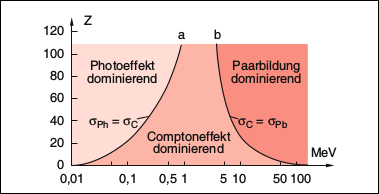
\includegraphics[width=6.8cm]{FCP_Z.png}
		\caption{Die dominanten Bereiche für Photoeffekt, Compton-Effekt und Paarbildung als Funktion der Ordnungszahl Z des Absorbers und der Energie $ E_{\gamma} $ der $ \gamma $ - Quanten}
	\end{subfigure}
	\begin{subfigure}{\textwidth}
		\centering
		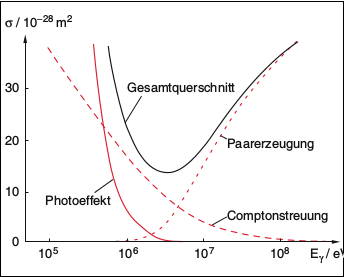
\includegraphics[width=6.8cm]{FCP_sigma.png}
		\caption{Wirkungsquerschnitt $ \sigma_{\text{Ph}} $ für Photoeffekt, $ \sigma_{C} $ für Compton--Effekt, und $ \sigma_{\text{Pb}} $ für Paarbildung für Blei (Z=82) als Funktion der $ \gamma $ -Energie}
	\end{subfigure}
	\caption{Vergleich von Photoeffekt, Compton-Effekt und Paarbildung im Hinblick auf (a) Kernladungszahl (b) Wirkungsquerschnitt}
\end{figure}
\clearpage
\thispagestyle{empty}
\begin{sidewaystable}[h]
    \centering\setlength\tabcolsep{1pt}
        \begin{tabular} {p{1.6cm} | c | p{3.5cm} | p{4cm} | p{5cm} | p{5.5cm} } 
             \textbf{Strahlung} &\textbf{Name} &\textbf{Bedingung} & \centering \textbf{$\derive{E}{x}$} & \textbf{Sonstiges} & \textbf{Wirkungsquerschnitt} \\ 
 			\midrule
              Elektron & Bremsstrahlung & $E \geq 580 \frac{MeV}{Z} $ & $\derive{E}{x} = \frac{E}{X_0} $ \newline \newline mit $X_0$ : Empirische Länge, abhängig von Absorbermaterial Länge nach der E auf $ \nicefrac{1}{e} $ abgefallen ist (Strahlungslänge)  &  \centering Kern für Impulsübertrag nötig  & $ \sigma_{\text{Br}} \propto \frac{Z \alpha^3}{(m_e c^2)^2} $ \newline Bei schwereren Teilchen sehr klein, daher irrelevant. \\ 
              \hline
              
              Schwere \newline Teilchen \newline Elektronen & Ionisation & & Bethe-Formel (\ref{bethe-formel}) \newline
              mit Z: Kernladungszahl\newline I: Anregungspotential \newline $ n = \frac{Z \rho}{Au} $ Elektronendichte des Absorbers \newline (bei kleinem Impuls $ \derive{E}{x} \propto \frac{1}{\beta^2} $ ) & Ionisationsenergie des Mediums: \newline $ I \approx (10Z+1) $ eV \newline \newline 
              Reichweite: \newline  $ R = \int_{E_{kin}} ^0 \frac{1}{\nicefrac{\md E}{\md x}} \md E $ & \\ 
              \hline 
              
              Schwere \newline Teilchen & Pion-Erzeugung & $ E = \sqrt{S} \geq 2m_p c^2 + m_{\pi} c^2 \newline  = 2m_p c^2 + 140 $ MeV & & Starke Wechselwirkung \newline Wenn Pionen andere Wechselwirkungen induzieren \newline Hadronenschauer mit Länge \newline $ \lambda_{int} = \frac{1}{\rho_{a} \sigma_{na}} $ \newline \newline Nukleare Wechselwirkungslänge & 30 mb für $ \sqrt{S} = 10 $ GeV \newline 80 mb für $ \sqrt{S} = 10 $ TeV \\ 
              \hline
              
              Photon & Photoeffekt & $E_{\gamma} \in [10 keV,1 MeV] $ & & & $ \sigma_{\text{Ph}} \propto \frac{Z^5}{\sqrt{E_{\gamma}}} $ \\ 
              \hline
              
              Photon & Comptoneffekt & $h \nu \gg I$ & & $ - \frac{1}{E_{\gamma}^{'}} - \frac{1}{E_{\gamma}} = \frac{1 - cos \theta}{m_e c^2}  \leq \frac{2}{m_e c^2} $ & $ \sigma_{C} \propto \frac{\alpha Z^2}{E_{CM}} $ 
             \newline \newline mit  \newline $ E_{CM} = \sqrt{(m_e c^2)^2 + 2 E_{\gamma} m_e c^2} $ \newline \newline $ \sigma_{C} = \pi r_E^2 Z \frac{m_e c^2}{E_{\gamma}} \left( \text{ln}  \left(\frac{2 E_{\gamma}}{m_e c^2}  + \frac{1}{2} \right) \right)$ \\ 
              \hline
              
              Photon & Paarbildung & $ E_{\gamma} \geq 2 m_e c^2$ & & & $ \sigma_{P} \propto Z^2 \  \ln (E_{\gamma}) $ \\
           \bottomrule
        \end{tabular}\hspace*{-1cm}
        \caption{Zusammenfassung und Ergänzungen}
\end{sidewaystable}

\end{document}